% @HEADER
% ***********************************************************************
% 
%            Trilinos: An Object-Oriented Solver Framework
%                 Copyright (2001) Sandia Corporation
% 
% Under terms of Contract DE-AC04-94AL85000, there is a non-exclusive
% license for use of this work by or on behalf of the U.S. Government.
% 
% This library is free software; you can redistribute it and/or modify
% it under the terms of the GNU Lesser General Public License as
% published by the Free Software Foundation; either version 2.1 of the
% License, or (at your option) any later version.
%  
% This library is distributed in the hope that it will be useful, but
% WITHOUT ANY WARRANTY; without even the implied warranty of
% MERCHANTABILITY or FITNESS FOR A PARTICULAR PURPOSE.  See the GNU
% Lesser General Public License for more details.
%  
% You should have received a copy of the GNU Lesser General Public
% License along with this library; if not, write to the Free Software
% Foundation, Inc., 59 Temple Place, Suite 330, Boston, MA 02111-1307
% USA
% Questions? Contact Michael A. Heroux (maherou@sandia.gov) 
% 
% ***********************************************************************
% @HEADER
\chapter{Multilevel Preconditioners with ML}
\label{chap:ml}

\ChapterAuthors{Marzio Sala, Michael Heroux, David Day}

\begin{introchapter}
The ML package defines a class of preconditioners based on multilevel
methods~\cite{Briggs2000,TuminaroTong:00a}. 
While theoretically ML preconditioners apply to any linear system,
the range of applicability of the methods is limited at this time,
primarily to certain linear elliptic partial differential equations
descretized with linear shape functions.
The ML package provides multilevel solvers and preconditioners based on
geometric and algebraic coarsening schemes.
Please contact the developers for information on the status of special purpose
methods, such as those for the incompressible Navier-Stokes equations
and Maxwell's equations.

This Chapter will present:
\begin{itemize}
\item A multilevel preconditioning framework (in Section~\ref{ml:theoretical});
\item How to use ml objects as AztecOO preconditioners (in
  Section~\ref{sec:ml_prec});
\item The ML\_Epetra::MultiLevelOperator class (in
  Section~\ref{sec:ml:operator});
\item How to define black-box preconditioners using the
  ML\_Epetra::MultiLevelPreconditioner Class (in
  Section~\ref{sec:ml:preconditioner});
\item How to implement two level domain decomposition methods with
  aggregation based coarse matrix (in Section~\ref{sec:ml_DD}).
\end{itemize}
\end{introchapter}

%%%
%%%
%%%
%%%
\section{A Multilevel Preconditioning Framework}
\label{ml:theoretical}
For certain combinations of iterative methods and linear systems, the
error at each iteration projected onto the eigenfunctions has components
that decay at a rate proportional to the corresponding eigenvalue (or
frequency).  Multilevel methods exploit this property \cite{Briggs2000}
by projecting the linear system onto a hierarchy of increasingly
coarsened ``meshes" so that each error component rapidly decays on at
least one coarse ``mesh."  The linear system on the coarsest ``mesh",
called the coarse grid problem, is solved exactly.  The iterative method
is called the smoother, as a reflection of its diminished role as a way
to damp out the high frequency error.  The grid transfer (or
interpolation) operators are called restriction ($\mathbf{R}$) and
prolongation ($\mathbf{P}$) operators.

Multilevel methods are characterized by 
the sequence of coarse spaces, 
the definition of the operator each coarse space,
the specification of the smoother, and the 
restriction and prolongation operators.
Geometric multigrid (GMG) methods  are multilevel methods 
that require the user to specify the underlying grid, and
in most cases a hierarchy of (not necessarily nested) coarsens grids.
Both the automatic generation of a grid-hierarchy for GMG and the 
specification of the ML, designed for unstructured problems,
are beyond the scope of the tutorial.

Algebraic multigrid (AMG)  (see \cite[Section 8]{Briggs2000}) 
method development has been motivated by the demand for multilevel
methods that are easier to use.
In AMG, both the matrix hierarchy and the prolongation operators are
constructed just from the stiffness matrix.  
Recall that to use Aztec00 or IFPACK,  a user must 
supply a linear system, and select a preconditioning strategy.
In AMG, the only additional information required 
from the user is to specify a coarsening strategy.

Readers that are unfamiliar with multigrid methods are strongly advised to
review \cite{Briggs2000} before using ML.

A multilevel method for (\ref{eq:linear_sys}) 
depends on the number of coarsen grid levels, 
and operators for each level.
Levels are numbered from the coarsest level, $0$, to the finest.
The pre- and post- smoothers  are denoted
${\bf S}_k^{(1)}$ and ${\bf S}_k^{(2)}$ respectively.
${\bf R}_{k-1,k}$
is the restriction operator from level $k$ to $k-1$, and ${\bf P}_{k,k-1}$ is a
prolongator from $k-1$ to $k$.
In AMG, the operators on the coarse meshes ${\bf A}_k$ are defined by
\[
{\bf A}_{k-1} = {\bf R}_{k-1,k} {\bf A}_k {\bf P}_{k,k-1}.
\]
The AMG coarse grid operators may be less sparse than the corresponding GMG coarse grid operators,
defined by assembling the coefficient matrix on the coarse grid.
These pieces combine into a multigrid solver.
\begin{center}
  Recursive Definition of the V-cycle Scheme {\tt MGM}( $x$, $b$, Number
  of Levels)
\end{center}
\begin{tabbing}
{\tt if} \= $k>0$ \\
\> $x = {\bf S}_k^{(1)} (x, b)$ \\
\> $d = {\bf R}_{k-1,k}(b - {\bf A}_k x)$\\
\> $v = {\bf 0}$ \\
\> {\tt MGM}( $v$, $d$, $k-1$) \\
\> $x = x + {\bf P}_{k,k-1} v $\\
\> $x = {\bf S}_k^{(2)}( x, b )$\\
{\tt else} \\
\> $x = {\bf A}_k^{-1} b $\\
\end{tabbing}
\begin{remark}
The tutorial only discussed AMG methods.
The interested reader is referred to 
\cite{ML-home-page} for information on GMG methods
in ML.
\end{remark}
%%%
%%%
%%%
\section{ML Objects as AztecOO Preconditioners}
\label{sec:ml_prec}
ML may be used as a ``black-box'' multilevel preconditioner, 
using aggregation procedures to define the multilevel hierarchy. 
In order to use ML as a preconditioner, we need to define an
AztecOO Solver, as outlined in Section~\ref{chap:aztecoo}. 
ML requires the user to define a structure that stores internal data.
The convention in ML is to call the structure \verb!ml_handle!.
Next define the maximum number of levels, 
the amount of diagnostic information written to the screen, 
which varies from none ($0$) to extremely verbose ($10$), 
and creaste the ML handle structure:
\begin{verbatim}
ML *ml_handle;
int N_levels = 10;
ML_Set_PrintLevel(3);
ML_Create(&ml_handle,N_levels);
\end{verbatim}

Next construct an ML preconditioner for an Epetra matrix.
Additionally, ML requires a structure that stores 
information about the aggregates at each level called ML\_Aggregate:
\begin{verbatim}
EpetraMatrix2MLMatrix(ml_handle, 0, &A);
ML_Aggregate *agg_object;
ML_Aggregate_Create(&agg_object);
\end{verbatim}

The multilevel hierarchy is constructed with the instruction
\begin{verbatim}
N_levels = ML_Gen_MGHierarchy_UsingAggregation(ml_handle,
                                               0,
                                               ML_INCREASING,
                                               agg_object);
\end{verbatim}
Here, \verb!0! is the index of the finest level, and the index of
coarser levels will be obtained by incrementing this value.
Please see \cite{ML-Users-Guide} for more information on the input parameters.

Next define the smoother, such as symmetric Gauss-Seidel,
and initialize the solver:
\begin{verbatim}
ML_Gen_Smoother_SymGaussSeidel(ml_handle, ML_ALL_LEVELS,
                               ML_BOTH, 1, ML_DEFAULT);
ML_Gen_Solver (ml_handle, ML_MGV, 0, N_levels-1);
\end{verbatim}

Finally, use this ML hierarchy to create an Epetra\_Operator, 
set the preconditioning operator of our AztecOO solver,
and then call \verb!Iterate()! as usual:
\begin{verbatim}
ML_Epetra::MultiLevelOperator MLop(ml_handle,comm,map,map);
solver.SetPrecOperator(&MLop);
solver.Iterate(Niters, 1e-12);
\end{verbatim}
The entire code is reported in 
\newline
\TriExe{ml/ex1.cpp}. 
The output is reported below.
\begin{verbatim}
[msala:ml]> mpirun -np 2 ./ex1.exe
**************************************************************
* ML Aggregation information                                 *
==============================================================
ML_Aggregate : ordering           = natural.
ML_Aggregate : min nodes/aggr     = 2
ML_Aggregate : max neigh selected = 0
ML_Aggregate : attach scheme      = MAXLINK
ML_Aggregate : coarsen scheme     = UNCOUPLED
ML_Aggregate : strong threshold   = 0.000000e+00
ML_Aggregate : P damping factor   = 1.333333e+00
ML_Aggregate : number of PDEs     = 1
ML_Aggregate : number of null vec = 1
ML_Aggregate : smoother drop tol  = 0.000000e+00
ML_Aggregate : max coarse size    = 1
ML_Aggregate : max no. of levels  = 10
**************************************************************
ML_Gen_MGHierarchy : applying coarsening
ML_Aggregate_Coarsen begins
ML_Aggregate_CoarsenUncoupled : current level = 0
ML_Aggregate_CoarsenUncoupled : current eps = 0.000000e+00
Aggregation(UVB) : Total nonzeros = 128 (Nrows=30)
Aggregation(UC) : Phase 0 - no. of bdry pts  = 0
Aggregation(UC) : Phase 1 - nodes aggregated = 28 (30)
Aggregation(UC) : Phase 1 - total aggregates = 8
Aggregation(UC_Phase2_3) : Phase 1 - nodes aggregated = 28
Aggregation(UC_Phase2_3) : Phase 1 - total aggregates = 8
Aggregation(UC_Phase2_3) : Phase 2a- additional aggregates = 0
Aggregation(UC_Phase2_3) : Phase 2 - total aggregates = 8
Aggregation(UC_Phase2_3) : Phase 2 - boundary nodes   = 0
Aggregation(UC_Phase2_3) : Phase 3 - leftovers = 0 and singletons = 0
 Aggregation time       = 1.854551e-03
Gen_Prolongator : max eigen = 1.883496e+00
ML_Gen_MGHierarchy : applying coarsening
ML_Gen_MGHierarchy : Gen_RAP
RAP time for level  0 = 5.319577e-04
ML_Gen_MGHierarchy : Gen_RAP done
ML_Gen_MGHierarchy : applying coarsening
ML_Aggregate_Coarsen begins
ML_Aggregate_CoarsenUncoupled : current level = 1
ML_Aggregate_CoarsenUncoupled : current eps = 0.000000e+00
Aggregation(UVB) : Total nonzeros = 46 (Nrows=8)
Aggregation(UC) : Phase 0 - no. of bdry pts  = 0
Aggregation(UC) : Phase 1 - nodes aggregated = 6 (8)
Aggregation(UC) : Phase 1 - total aggregates = 2
Aggregation(UC_Phase2_3) : Phase 1 - nodes aggregated = 6
Aggregation(UC_Phase2_3) : Phase 1 - total aggregates = 2
Aggregation(UC_Phase2_3) : Phase 2a- additional aggregates = 0
Aggregation(UC_Phase2_3) : Phase 2 - total aggregates = 2
Aggregation(UC_Phase2_3) : Phase 2 - boundary nodes   = 0
Aggregation(UC_Phase2_3) : Phase 3 - leftovers = 0 and singletons = 0
 Aggregation time       = 1.679042e-03
Gen_Prolongator : max eigen = 1.246751e+00
ML_Gen_MGHierarchy : applying coarsening
ML_Gen_MGHierarchy : Gen_RAP
RAP time for level  1 = 4.489557e-04
ML_Gen_MGHierarchy : Gen_RAP done
ML_Gen_MGHierarchy : applying coarsening
ML_Aggregate_Coarsen begins
Aggregation total setup time = 8.903003e-02 seconds
Smoothed Aggregation : operator complexity = 1.390625e+00.

           *******************************************************
           ***** Preconditioned CG solution
           ***** Epetra ML_Operator
           ***** No scaling
           *******************************************************

           iter:    0           residual = 1.000000e+00
           iter:    1           residual = 1.289136e-01
           iter:    2           residual = 4.710371e-03
           iter:    3           residual = 7.119470e-05
           iter:    4           residual = 1.386302e-06
           iter:    5           residual = 2.477133e-08
           iter:    6           residual = 6.141025e-10
           iter:    7           residual = 6.222216e-12
           iter:    8           residual = 1.277534e-13


           Solution time: 0.005845 (sec.)
           total iterations: 8
Residual    = 6.99704e-13
\end{verbatim}
%%%
%%%
%%%
\section{The ML\_Epetra::MultiLevelOperator Class}
\label{sec:ml:operator}
As with other Trilinos packages, ML can be compiled and run independently
from Epetra. It accepts input matrix in formats different
from the Epetra\_RowMatrix or Epetra\_Operator. However, as part of the
Trilinos project, ML can be used to define a preconditioner operator for
\verb!Epetra_LinearProblem! objects (see for
instance~\cite{Epetra-Ref-Guide-new}). This means that, in a C++ framework,
ML can be defined as an \verb!Epetra_Operator! object, applied to an
\verb!Epetra_MultiVector!  object, and used as a preconditioner for
AztecOO.  This can be done in two ways:
\begin{itemize}
\item By defining an \verb!ML_Epetra::MultiLevelOperator! object, derived from the
  Epetra\_\-Operator class. The constructor of this object requires
  already filled ML\_Struct and ML\_Aggregate structures.  ML must have
  been configure with the option \newline \verb!--enable-epetra!.
\item By defining an \verb!ML_Epetra::MultiLevelPreconditioner! object, derived
  from the Epetra\_RowMatrix class. Basically, the constructor of
  this object demands for an Epetra\_RowMatrix  pointer and a
  Teuchos parameter list, that contains all the user's defined
  parameters. ML must have been configure with options \newline
  \verb!--enable-epetra --enable-teuchos!.
\end{itemize}

The first approach, described in Section~\ref{sec:ml:operator}, is more
general, and can be applied to geometric and algebraic multilevel
preconditioner, but it requires a deeper knowledge of the ML package.
This is because the user has to explicitly construct the ML hierarchy,
define the aggregation strategies, the smoothers, and the coarse grid
solver. The second approach, presented in
Section~\ref{sec:ml:preconditioner}, instead, although limited to algebraic
multilevel preconditioners, allows the use of ML as a black-box
preconditioner. This class automatically constructs all the components
of the preconditioner, following the parameters specified in a Teuchos
parameters' list. 

Next we walk through how to write some code to
construct an ML preconditioner for an \verb!Epetra_RowMatrix! $A$.
The \verb!ML_Epetra::MultiLevelOperator! class 
is defined in the header file \verb!ml_MultiLevelOperator.h!.
Users must include it, and along with some subset of
\verb!ml_config.h!,
\verb!AztecOO.h!,
\verb!Epetra_Operator.h!, 
\verb!Epetra_MultiVector.h!
and
\verb!Epetra_-!
\verb!LinearProblem.h!.
Check the Epetra and AztecOO documentation for more information on this topic.

The next steps proceed exactly as in \S~\ref{sec:ml_prec}:
\begin{verbatim}
ML *ml_handle;
int N_levels = 10;
ML_Set_PrintLevel(3);
ML_Create(&ml_handle,N_levels);
EpetraMatrix2MLMatrix(ml_handle, 0, &A);
ML_Aggregate *agg_object;
ML_Aggregate_Create(&agg_object);
N_levels = ML_Gen_MGHierarchy_UsingAggregation(ml_handle, 
                                               0,
                                               ML_INCREASING,
                                               agg_object);
ML_Gen_Smoother_SymGaussSeidel(ml_handle, ML_ALL_LEVELS,
                               ML_BOTH, 1, ML_DEFAULT);
ML_Gen_Solver (ml_handle, ML_MGV, 0, N_levels-1);
ML_Epetra::MultiLevelOperator MLop(ml_handle,comm,map,map);
\end{verbatim}

At this point, our example diverges from \S~\ref{sec:ml_prec}.
Instead of using ML to solve the linear system $A x = b$,
where $x$ and $b$ are \verb!Epetra_MultiVector!,  use 
the ML operator as the precondition for an Aztec00 linear system,
and solve it:
\begin{verbatim}
Epetra_LinearProblem Problem(A,&x,&b);
AztecOO Solver(Problem);
Solver.SetPrecOperator(&MLop);
Solver.SetAztecOption( AZ_solver, AZ_gmres );
Solver.Iterate(Niters, 1e-12);
\end{verbatim}
%%%
%%%
%%%
\section{The ML\_Epetra::MultiLevelPreconditioner Class}
\label{sec:ml:preconditioner}
An alternative to the ML\_Epetra::MultiLevelOperator
(that is also in the namespace {\tt ML\_Epetra}) 
is the \verb!MultiLevelPreconditioner! class.  Replace the header file 
\newline \verb!ml_MultiLevelOperator.h!  discussed in section~\ref{sec:ml:operator} 
by \verb!ml_MultiLevelPreconditioner.h!.

Table~\ref{tab:ml:aggr} reports the aggregation schemes currently
available in ML. 
%A graphical comparison of Uncoupled and METIS is
%reported in Figure~\ref{fig:ml:comparison}, for a
%Laplacian operator over a square descretized with a a $9$ point stencil.

%\begin{figure}[htbp]
  %\centering
  %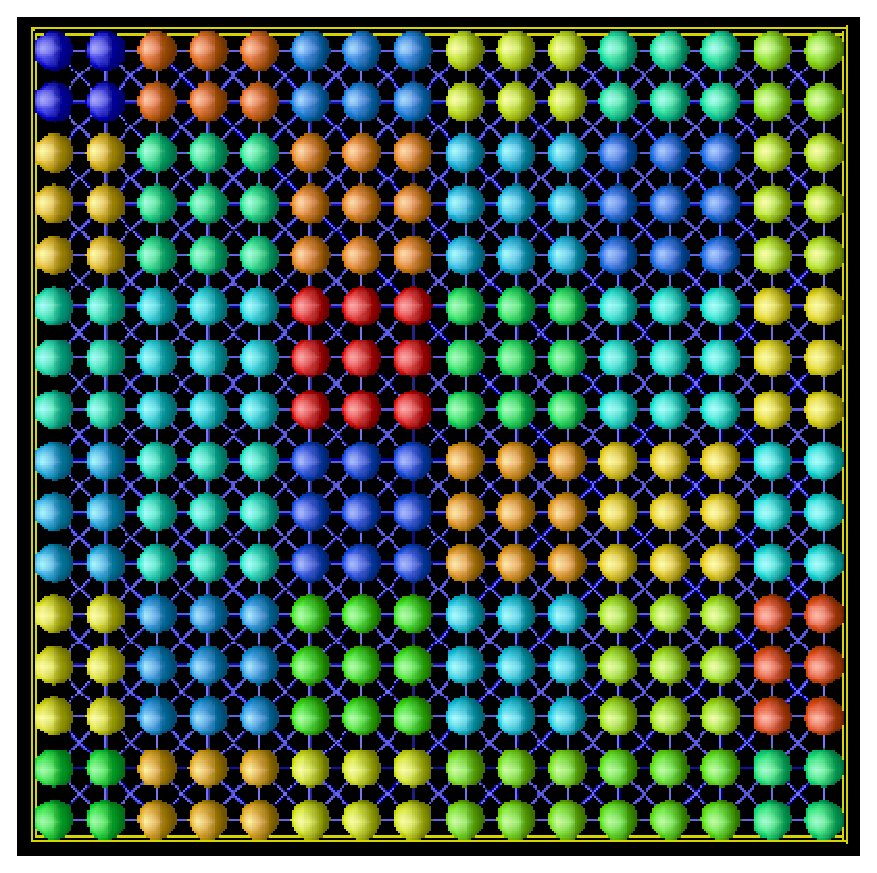
\includegraphics[height=6cm]{ml_Uncoupled-16x16.ps} \hspace{0.5cm}
  %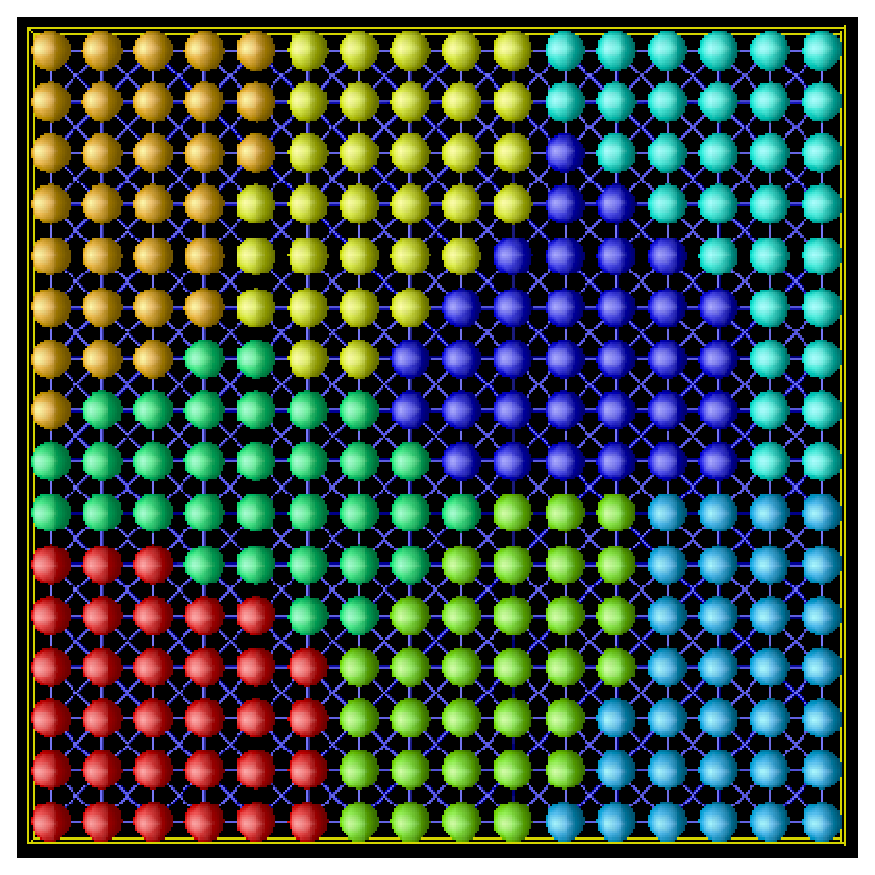
\includegraphics[height=6cm]{ml_METIS-16x16.ps}
  %\caption{Aggregates for Uncoupled (left) and METIS (right) for a 16x16 Cartesian grid.}
  %\label{fig:ml:comparison}
%\end{figure}

\begin{table}
\begin{center}
\begin{tabular}{ | p{5cm} | p{10cm} | }
\hline
\verb!Uncoupled! & For a $1$,$2$,or $3$ dimensional structured Cartesian grid 
                   with a $3$, $9$ or $27$ point stencil respectively,
                   construct aggregates of optimal size such that
                   each aggregate resides on one processor.\\
\verb!MIS! & Maximal independent set based coarsening with aggregates
             allowed to reside on multiple processes. 
             The scheme minimizes the number of iterations,
             but the cost per iteration is high.  \\
\verb!METIS! & Use a serial graph partitioner to create
               aggregates residing on one processor. 
               The number of nodes in each aggregate
               is specified with the option {\tt aggregation: nodes per aggregate}.
               ML must be configured with {\tt --with-ml\_metis}. \\
\verb!ParMETIS! & Use a parallel graph partitioner to create aggregates that
                  may reside on multiple processors.  
                  ML must be configured with {\tt --with-ml\_parmetis3x}. 
                  The number of aggregates is
                  specified by option {\tt aggregation: global number}. \\
\hline
\end{tabular}
\caption{ML\_Epetra::MultiLevelPreconditioner Coarsening Schemes}
\label{tab:ml:aggr}
\end{center}
\end{table}

\begin{table}
\begin{center}
\begin{tabular}{ | p{5cm} | p{10cm} | }
\hline
\verb!Jacobi! & Point-Jacobi. Damping factor is specified using
{\tt smoother: damping factor}, and the number of sweeps with {\tt
  smoother: sweeps} \\ 
\verb!Gauss-Seidel! & Point Gauss-Seidel. \\
\verb!Aztec! & Use AztecOO's built-in preconditioning functions as
smoothers. Or, use approximate solutions with AztecOO as smoothers. 
The AztecOO vectors \verb!options! and {\tt params} can be set using
{\tt smoother: Aztec options} and {\tt smoother: Aztec params}. \\
\hline
\end{tabular}
\caption{ML\_Epetra::MultiLevelPreconditioner Smoothers} 
\label{tab:ml:smoother}
\end{center}
\end{table}

\begin{table}
\begin{center}
\begin{tabular}{ | p{5cm} | p{10cm} | }
\hline
\verb!Jacobi! & Use Jacobi as a solver. \\
\verb!Gauss-Seidel! & Use Gauss-Seidel as a solver. \\
\verb!Amesos_KLU! & Use Amesos's KLU sequential solver. \\
\verb!Amesos_UMFPACK! & Use UMFPACK. \\
\verb!Amesos_Superludist! & Use SuperLU\_DIST. \\
\verb!Amesos_MUMPS! & Use MUMPS. \\
\hline
\end{tabular}
\caption{ML\_Epetra::MultiLevelPreconditioner Coarsest Grid Exact Solvers
  To use Amesos, ML must be configured with {\tt --enable-amesos} 
  and Amesos also be configured as needed.}
\label{tab:ml:coarse}
\end{center}
\end{table}

A very simple fragment of code using this class is reported below.
The reader may refer to file
\verb!$ML_HOME/examples/ml_example_MultiLevelPreconditioner.cpp! for a more
complex example. To run example, first 
configure ML \verb!--enable-triutils!.
\begin{verbatim}
#include "ml_include.h"
#include "ml_MultiLevelPreconditioner.h"
#include "Teuchos_ParameterList.hpp"

...

  // A is an Epetra_RowMatrix derived class object
  // solver is an AztecOO object

  Teuchos::ParameterList MList;

  // default values for smoothed aggregation
  ML_Epetra::SetDefaults("SA",MLList);
  MLList.set("max levels",6);
  MLList.set("increasing or decreasing","decreasing");
  MLList.set("aggregation: type", "MIS");
  MLList.set("coarse: type","Amesos_KLU");
  
  ML_Epetra::MultiLevelPreconditioner * MLPrec = 
    new ML_Epetra::MultiLevelPreconditioner(A, MLList, true);

  solver.SetPrecOperator(MLPrec);
  solver.SetAztecOption(AZ_solver, AZ_gmres);
  solver.Iterate(Niters, 1e-12);

  ...

  delete MLPrec;
\end{verbatim}
The general procedure is as follows. First, the user defines a Teuchos
parameters' list. Second input parameters are set via method
\verb!set(ParameterName,ParameterValue)!, where \verb!ParameterName! is
a string defining the parameter, and \verb!ParameterValue! is the
specified parameter, that can be any C++ object or pointer.  This list
is passed to the constructor, together with a pointer to the matrix, and
a boolean flag.  If this flag is set to \verb!false!, the constructor
will not compute the multilevel hierarchy until when
{\tt MLPrec->ComputePrecon-}\newline {\tt ditioner()} is called. The hierarchy can be
destroyed using \verb!MLPrec->Destroy()!.  For instance, the user may
define a code like:
\begin{verbatim}
  // A is still not filled with numerical values
  ML_Epetra::MultiLevelPreconditioner * MLPrec = 
    new ML_Epetra::MultiLevelPreconditioner(A, MLList, false);
  
  // compute the elements of A
  ...
  // now compute the preconditioner
  MLPrec->ComputePreconditioner();

  // solve the linear system, and refill A
  ...
  MLPrec->Destroy(); // destroy previous preconditioner,
  MLPrec->ComputePreconditioner(); // and build a new one
\end{verbatim}
In this fragment of code, the user defines the ML preconditioner, but
does not create the preconditioner in the construction phase. This is of
particular interest, for example, when ML is used in conjunction with
nonlinear solvers (like NOX~\cite{NOX-home-page}).

We point out that the input parameter list is {\sl copied} in the
construction phase, hence later changes to \verb!MLList! will not affect
the preconditioner. Should one need to modify parameters in the
\verb!MLPrec!'s internally stored parameter list, proceed as
follows:
\begin{verbatim}
  ParameterList & List = MLPrec->GetList();
\end{verbatim}
and then directly modify \verb!List!.

\medskip

All ML options can have a common prefix, specified by the
user in the construction phase. For example, suppose that we require
\verb!ML: ! to be the prefix. The constructor will be
\begin{verbatim}
  MLLIst.set("ML: aggregation: type", "METIS");
  ML_Epetra::MultiLevelPreconditioner * MLPrec = 
  new ML_Epetra::MultiLevelPreconditioner(*A,  
                                          MLList, 
                                          true, 
                                          Prefix);
\end{verbatim}
where \verb!Prefix! is a char array containing \verb!ML: !.

Note that spaces are important: Do not include leading or trailing
spaces, and separate words by just one space! Misspelled parameters will
not be used, and can be detected calling method \verb!PrintUnused()!
{\sl after} the construction of the multilevel hierarchy. 

For a detailed list of all the parameters, we refer to the ML user's
guide.  Here, we report the most used parameters in
Tables~\ref{tab:ml:aggr}, \ref{tab:ml:smoother} and \ref{tab:ml:coarse}.


%%%
%%%
%%%


\section{Two-Level Domain Decomposition Preconditioners with ML}
\label{sec:ml_DD}

The idea of two level domain decomposition based on aggregation is to
use a graph partitioner to partition the local or global graph into
subgraphs, and then treat each subgraph as a large aggregate.

The example contained herein 
uses the graph decomposition library METIS to create the coarse-level matrix.
If you don't have METIS, or just do not want to
re-configure ML, you may run the example 
you will be limited to use only one aggregate per process.
There are three changes to the Trilinos configuration.
One flag tells the package (ML) to look for an external library,
and the other two flag tells the compiler
where to find the include directories and external library.
Configure ML with the flags \verb!--with-ml_metis!,
and with {\tt --with-incdirs} and {\tt --with-ldflags}
set to the locations of the METIS include files and library. 
Please type {\tt configure --help} in the ML subdirectory for more information. 

Two-level domain decomposition methods are
effective for the iterative solution of many different kinds of linear
systems.  For some classes of problems, a very convenient way to define
the coarse grid operator is to use an aggregation procedure. This is very
close to what presented in Section~\ref{sec:ml_prec}. The main
difference is that only two level methods are considered, and that the
coarse grid remains of (relatively) small size. The idea is to define a
small number of aggregates on each process, using a graph decomposition
algorithm (as implemented in the library METIS, for
instance)\footnote{Aggregation schemes based on ParMETIS are also
available. Please refer to the help of the ML {\tt configure} for more
details.}. This can be done as follows.

The linear system matrix \verb!A!, here coded as an
Epetra\_CrsMatrix\footnote{Epetra\_VbrMatrix and Epetra\_RowMatrix can
  be used as well.}, corresponds to the descretization of a 2D Laplacian
on a Cartesian grid. \verb!x! and \verb!b! are the solution vector and
the right-hand side, respectively.

The AztecOO linear problem is defined as
\begin{verbatim}
  Epetra_LinearProblem problem(&A, &x, &b);
  AztecOO solver(problem);
\end{verbatim}

At this point, we can create the Teuchos parameters' list, with the
following parameters:
\begin{verbatim}
  ParameterList MLList;

  ML_Epetra::SetDefaults("DD",MLList);

  MLList.set("max levels",2);
  MLList.set("increasing or decreasing","increasing");

  MLList.set("aggregation: type", "METIS");
  MLList.set("aggregation: nodes per aggregate", 16);
  MLList.set("smoother: pre or post", "both");
  MLList.set("coarse: type","Amesos_KLU");
  MLList.set("smoother: type", "Aztec");
\end{verbatim}
The last option tells ML to use the Aztec preconditioning function as a
smoother. Aztec requires an integer vector \verb!options! and a double
vector \verb!params!. Those can be defined as follows:
\begin{verbatim}
  Teuchos::RCP<vector<int>> options = rcp(new vector<int>(AZ_OPTIONS_SIZE));
  Teuchos::RCP<vector<double>> params = rcp(new vector<double>(AZ_PARAMS_SIZE));
  AZ_defaults(options,params);
  AZ_defaults(&(*options)[0],&(*params)[0]);
  (*options)[AZ_precond] = AZ_dom_decomp;
  (*options)[AZ_subdomain_solve] = AZ_icc;

  MLList.set("smoother: Aztec options", options);
  MLList.set("smoother: Aztec params", params);
\end{verbatim}
The last two commands set the Teuchos reference-counted pointers,
{\tt options} and {\tt params}, in the parameter list.
Note that {\sl all} Aztec preconditioners can be used as smoothers for
ML. 
At this point we can create the ML preconditioner as
\begin{verbatim}
  ML_Epetra::MultiLevelPreconditioner * MLPrec =
    new ML_Epetra::MultiLevelPreconditioner(A, MLList, true);
\end{verbatim}
and check that no options have been misspelled, using
\begin{verbatim}
  MLPrec->PrintUnused();
\end{verbatim}
AztecOO solver is called using
\begin{verbatim}
  solver.SetPrecOperator(MLPrec);

  solver.SetAztecOption(AZ_solver, AZ_cg_condnum);

  int Niters = 500;
  solver.SetAztecOption(AZ_kspace, 160);

  solver.Iterate(Niters, 1e-12);
\end{verbatim}
Finally, some (limited) information about the preconditioning phase are
obtained using
\begin{verbatim}
  cout << MLPrec->GetOutputList();
\end{verbatim}
The entire code is reported in 
\newline
\TriExe{ml/ex2.cpp}.
\newline
